\newpage
\section*{Zielsetzung}
Es soll die Compton-Wellenlänge $\lambda_c$ des Elektrons bestimmt werden.
\section{Theorie}
\subsection{Die Compton-Strahlung}
\label{sec:theorie}
Trifft Röntgenlicht mit einer Wellenlänge $\lambda_1$ auf ein schwach gebunden Elektron, so enthält das gestreute Licht eine neue 
größere Wellenlänge $\lambda_2$, da das Photon einen Teil seiner Energie durch den elastischen Stoß
an das Elektron übertragten hat. 
Dies folgt aus 
\begin{equation}
    E_{Photon}=\frac{hc}{\lambda}.
    \label{eqn:energie}
\end{equation}
Zusätzlich wird diese Wellenenlänge um den Winkel $\Theta$ abgelenkt.
Die Wellenlängenverschiebung $\Delta \lambda$ und der Streuungswinkel 
$\Theta$ weisen folgenden Zusammhang auf
\begin{equation}
    \Delta \lambda = \lambda_2 - \lambda_1 =\frac{h}{m_e c}\left(1-cos(\Theta)\right)=\lambda_c \cdot \left(1-cos(\Theta)\right).
    \label{eqn:compton}
\end{equation}
Die Konstante $\lambda_c$ nennt man die Compton-Wellenlänge des Elektrons.
\begin{figure}[H]
    \centering
    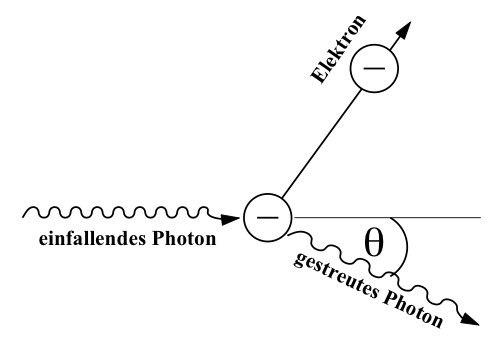
\includegraphics[width=0.4\textwidth]{compton/compton_effekt.jpg}
    \caption{Darstellung des Compton Effekts mit einem einfallendem Photon, dass
    auf ein Elektron trifft. Das gestreute Photon wird um den Winkel $\Theta$
    abgelenkt.\cite[1]{anleitung}}
\end{figure}
Man spricht von einer Reflexion bei $\Theta=\pi$, dabei wird die Wellenlängendifferenz
$\Delta \lambda$ maximal (vgl. Gl. \ref{eqn:compton}).

Der Compton-Effekt kann bei allen Photonen verschiedenster Energien beobachtet werden.
Die Wahrscheinlichkeit für das Auftetten ist allerdings bei hochenergetische Photonen wie
Rönten- oder $\gamma$-Strahlung am höchsten.
\newpage
\subsection{Erzeugung der Röntenstrahlung}
Zur Erzeugung nutze man die Eigenschaft der Bremstrahlung sowie die charakteristische
Röntgenstrahlung.\\ 
Eine Glühkathode emittiert dabei Elektronen, die durch eine evakuierte Röhre auf 
eine Annode hin beschleunigt werden. 
Beim Auftreffen auf die Annode wird Röntgenstrahlung ausgesendet.
Das ausgesendete Spektrum besteht aus charakteristischen Peaks, welche vom
Anodenmaterial abhängig sind und einem kontinuierlichen Bremsspektrum.

\subsubsection*{Charakteristische Strahlung}
Die Charakteristische Strahlung hängt vom Annodenmaterials ab. Durch das Auftreffen
der beschleunigten Elektron kann eine Energieübertragung an die im Material gebunden Elektronen stattfinden.
Die gebunden Elektronen können darauf hin auf ein höheres Energieniveau angeregt werden bevor 
sie wieder auf ein niedriges Energienivea zurückspringen. Dabei wird Strahlung frei,
dessen Energie der Energiedifferenz der verschiedenen Niveaus entspricht.

\subsubsection*{Bremsstrahlung}
Wird ein Elektron mithilfe eines elektrischen Feldes abgebremst, erfährt es eine
Beschleunigung und verliert somit kinetische Energie. Diese Energie wird in Form von
Röntgenphotonen ausgesendet. Hierbei bildet sich ein kontinuierliches Spektrum aus.


\subsection{Bragg-Reflektion (Bestimmung der Röntgenwellenlänge)}
Über die Bragg'sch Reflektion kann die Energie $E$ der Röntgenstrahlung analysiert werden.
Durch die Beugung der Strahlung an einem dreidimensionalen Gitter mit dem Gitterkonstante $d$ 
entsteht beim Glanzwinkel $\alpha$ eine konstruktive Interferenz. Die Wellenlänge bestimmt 
sich nun über den Zusammenhang
\begin{equation}
    2 d sin(\alpha)=n \lambda,
    \label{eqn:bragg}
\end{equation}
wobei $n$ die Beugungsordnung beschreibt.
\label{sub:bragg}

\begin{figure}
    \centering
    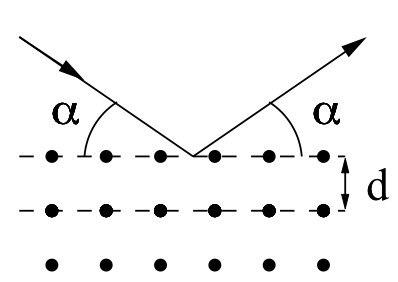
\includegraphics[width=0.35\textwidth]{plots/bragg.jpg}
    \caption{Die Bragg'sche Reflexion mit Braggwinkel $\alpha$ und 
    Gitterkonstante $d$.\cite[2]{anleitung}
    }
\end{figure}


\subsection{Geiger-Müller-Zählrohr}
Um die Impulsrate zu bestimmen, wird ein Geiger-Müller-Zählrohr verwendet.
Grundlegend besteht es aus einem mit Gas gefülltem Zylinder, dessen Wände die Kathode bilden.
Trifft nun isonisiernde Strahlung ein, so reagierte diese mit den Gasatomen. 
Die frei werdenen Elektronen werden durch die Annode als Impuls regestriert.
Damit das Gasatom wieder eine neutrale Ladung erhält, muss es zur Stabanode wandern.
Daraus folgt das Problem, wenn die Intensität der eintreffenden Strahlung zu hoch ist,
so sind bereits alle Atome ionsisiert und es folgt eine Verfälschung der Impulsrate.
Dies wird durch die Totzeit quantifiziert. Die beschreibt, wie lange es dauert bis
nach einem vergangenem Signal, das nächste Signal aufgenommen werden kann.
Diesen Fehler kann man durch folgende Formel korrigieren:

\begin{equation}
    I=\frac{N}{1-\tau \cdot N},
    \label{eqn:totzeit}
\end{equation}
dabei ist $N$ die Impulsrate und $\tau$ die Totzeit.